\documentclass{article}
\usepackage{presentation_notes}

\usepackage{geometry}
\geometry{margin=1in}


\title{Presentation notes} 
\author{Edmund Lau}
\date{\today}

\begin{document}
\maketitle


% ---------------------------- Section: Introduction
\section*{Abstract}

%In the analysis of partial differential equations, we are interested in the existence, uniqueness and regularity of the solutions. The Fredholm problem of a given differential operator asks the following question: Can we construct Banach spaces of a priori (weak) solutions between which the given operator acts as a Fredholm map? The Fredholm property will then reduce the question of existence and uniqueness to checking a finite number of conditions. For differential operators, such problems are typically solved with Sobolev spaces where regularity data of their elements are built into the Hilbert space structure, thus providing the link to regularity. \\
%\\
%Traditionally, Fredholm problems are associated with elliptic, i.e. essentially invertible, operators. However, there has been recent progress in non-elliptic setting using microlocal analysis. In this talk, we will introduce the central machineries of microlocal analysis, in particular, the propagation of singularity estimate  and use it to solve a particular non-elliptic Fredholm problem, which is  that of the wave operator on torus. 

In the analysis of partial differential equations, we are interested in the existence, uniqueness and regularity of the solutions. Given a linear differential operator, one typically asks the following question: can we construct Banach spaces of a priori (weak) solutions between which the given operator acts as a Fredholm map? The Fredholm property will then reduce the question of existence and uniqueness to finite dimensional linear algebra. For differential operators, such problems are frequently solved with Sobolev spaces where regularity data of their elements are built into their Hilbert space structure, thus providing the link to regularity. \\
\\
Traditionally, Fredholm problems are associated with elliptic operators. However, there has been recent progress in non-elliptic setting using microlocal analysis. In this talk, we will introduce the central machineries of microlocal analysis, in particular, the propagation of singularity estimate and use it to construct a non-elliptic Fredholm problem for a perturbation of the wave operator on the torus.



\section{Introduction}

First, the setup and some notations. A linear differential operator on $\R^n$ of order $k \in \N$, looks like 
\begin{align*}
P = \sum_{\abs{\alpha} \leq k} c_\alpha(x) D^\alpha_x = \sum_{\alpha \wh \alpha_1 + \dots \alpha_n \leq k} c_\alpha(x) \brac{-i \p_{x_1}}^{\alpha_1}\brac{-i \p_{x_2}}^{\alpha_2} \dots \brac{-i \p_{x_n}}^{\alpha_n}
\end{align*}
\todo{explain multi-index and $D$}. A partial differential equation of $P$ will look like
\begin{align*}
P u = f
\end{align*}
for some functions $u, f : \R^n \to \C$. Since we are taking upto $k$ derivatives, it seems reasonable to demand that $u \in C^k(\R^n)$, but turns out that's too restrictive and, in fact, there is a consistent way of talking solutions that need not even be continuous. We call these weak solutions or \emph{distributions}. These are linear functionals 
\begin{align*}
u : \sch(\R^n) \to \C
\end{align*}
e.g. the Dirac delta distribution $\delta(\varphi) = \varphi(0)$, $\varphi \in \sch(\R^n)$. We are mainly interested in tempered distributions because these are distribution where Fourier transform works and Fourier transform is central to microlocal analysis. 

Given a PDE, there are three immediate question that we are interested in: 
\begin{enumerate}
    \item Does a solution $u$ exists? 
    \item If it does, is it unique? 
    \item How regular is the solution? Is it a weak solution? Is it continuous? Is it differentiable? smooth? rapidly decaying? 
\end{enumerate}

Functional analysis, or of particular concern for us, the theory of Fredholm (differential) operators provides us with a way of tackling all three question simultaneously. In this this talk, we will 

\begin{itemize}
    \item see how being Freholm is link to existence, uniqueness and regularity. 
    \item briefly see why elliptic operators, which are essentially invertible operators, are Fredholm. \todo{mention that this is a typical and traditional case of study}
    \item There are non-elliptic Fredholm operators too! We will get our hands dirty and actually prove one. 
\end{itemize}
There are a couple of missing information in these statements which we will rectify along the way. Also along the way, we will introduce some relevant machineries from microlocal analysis \todo{name drop pseudodifferential operators here??} useful for such problems. \todo{refer to thesis for more complete development of microlocal analysis and pseudodifferential calculus.}

\todo{All the statements above needs some qualifying like compact manfold and domains codomainsn for Fredholms maps. This will be part of the content. }


\section{Fredholm Operators} 
So, we recall Fredholm maps. \todo{and an excuse to introduce spaces and notations for later.}
\begin{definition}[Fredholm operators]
    A continuous linear operator $T : \X \to\Y$ between Banach spaces $\X$ and $\Y$ is Fredholm, if 
    \begin{itemize}
        \item $T$ has closed range, i.e. $T(\X)$ is closed in $\Y$, 
        \item $\ker(T) \subset \X $ is finite dimensional, 
        \item $\coker(T) := \Y / T(\X)$ is finite dimensional. 
    \end{itemize}
\end{definition}

If we are given $y \in \Y$ and we want to solve for $x$ in $Tx = y$, then recall that for linear maps the ``size" of the kernel is a measure of non-uniqueness of solution $x$ and the cokernel is the amount of obstructions to solvability. More precisely, 
\begin{itemize}
    \item solvable if and only if  $y \not \in \coker(T)$. 
    \item unique if and only if $\ker(T) = 0$. 
\end{itemize}
The finite dimension property of the Fredholm maps thus reduces questions of existence and uniqueness of solutions to 
\begin{align*}
Pu = f
\end{align*}
to checking a finite number of conditions. And here we encounter our first piece of missing information: we can talk about a differential operator being Fredholm only when we have specify its domain and codomain, i.e. where $f$ lives and where we expect $u$ to belong. So, the question becomes
\begin{center}
    Given a $P$, can we construct $\X, \Y$ so that $P : \X \to \Y$ is Fredholm? 
\end{center}
For differential operators, we will want $\X, \Y$ to be spaces of distributions. This is known as ``constructing a Fredholm problem" for the operator $P$. In PDE, this is  frequently done with Sobolev spaces. 
\begin{fdefinition}[Sobolev Spaces]
    Given  $n, k \in \N$, the Sobolev space of order $k$ on $\R^n$ is 
    \begin{align*}
    H^k(\R^n) = \set{u \in L^2(\R^n) \wh D^\alpha u \in L^2(\R^n), \quad \abs{\alpha} \leq k}
    \end{align*}
    where $D^\alpha u $ is the distributional  derivative of $u$. Result from Fourier analysis shows that 
    \begin{align*}
    u \in H^k(\R^n) \iff \brac{1 + \abs{\xi}^2}^{k/2} \F u(\xi) \in L^2(\R^n)
    \end{align*}
    allowing using to generalise to arbitrary real order $s \in \R$, giving
    \begin{align*}
    H^s(\R^n) = \set{u \in \sch'(\R^n) \wh \brac{ 1 + \abs{\xi}^2}^{s/2} \F u \in L^2(\R^n)}. 
    \end{align*}
    We can give a Hilber space structure on $H^s(\R^n)$, by 
    \begin{align*}
    \inprod[u, v]_{H^s} = \inprod[ \Lambda^s u, \Lambda^sv]_{L^2}. 
    \end{align*}
    where $$\Lambda^su = \F^{-1}(\abrac{\xi}^s \hat{u})$$ is a topological isormophism $\Lambda^s : \sch' \to \sch'$. 
\end{fdefinition}

Sobolev spaces are important in PDE because they measures (global) regularity and decay. 
\begin{align*}
\norm[u]_{H^k} = \norm[u]_{L^2} + \sum_{\abs{\alpha} \leq k} \norm[D^\alpha u ]_{L^2} 
\end{align*}
\todo{First term sufficient decay and later terms boundedness in derivatives. Connect with Fourier analysis, intuition: Need arbitrarily high frequency wave to approximate jump discontinuity.} 

So, if we can construction Fredholm problem of the operator $P$ of the form
\begin{align*}
P : H^{s} \to H^{s'}
\end{align*}
for some $s, s'$ dependend on $P$, we will then have information about regularity of the solutions of $Pu = f$ as well. 


In practise, instead of topological statements, we translates properties like continuity and Fredholm into estimates. For continuity of an operator $T : \X \to \Y$, we have the familiar boundedness condition $\norm[Tx]_{\Y} \leq C \norm[x]_{\X}$ for all $u \in \X$. For Fredholm, we will need the following theorem. 
\begin{theorem} \label{theorem: fredholm estimates}
    Let $\X$, $\Y$, $\mathcal{Z}$ be Banach spaces.  If 
    \begin{itemize}
        \item $T : \X \to \Y$ is continuous, 
        \item $\X$ is compactly contained in $\mathcal{Z}$, i.e. the injection $\iota : \X\hookrightarrow \mathcal{Z}$ is compact, 
        \item for all $u \in \X$, there exist $C > 0$ such that the estimate 
        \begin{align*}
        \norm[x]_\X \leq C \brac{\norm[Tx]_\Y + \norm[u]_\mathcal{Z}}
        \end{align*}
        holds, 
    \end{itemize}
     then the image, $T(\X)$ is closed, and $T$ has finite dimensional kernel. 
\end{theorem}

For differential operators between Sobolev spaces, $P : H^s \to H^{s'}$,  the estimate we want is 
\begin{align*}
\norm[u]_{H^s} \leq C \brac{\norm[Pu]_{H^{s'}} + \norm[u]_{H^{N}}}. 
\end{align*}
The idea is that we can take $N$ to be highly negative, then, at least on compact manifold $M$ (such as the torus!), we have $H^s(M) \Subset H^N{M}$. \todo{For non-compact manifold or Euclidean $\R^n$ we will need weighted sobolev spaces and decay conditions for the operator. Need to mention the dual map.}


%
%\subsection{The Fredholm Index}
%Fredhol index of $T \in Fred(H_1, H_2)$ is locally constant over $T$. 
%
%\subsection{Fredholm differential operators between Sobolev Spaces}
%Elliptic operators on compact manifold. Ellipticity and isomorphism outside of the zero section
%

\section{Pseudodifferential operators and the elliptic ones} 
We have now relate Fredholm operators with existence, uniqueness and, importantly, regularity of its solutions and has reduced Fredholm conditions to estimates. The problem now is: How do we get those estimates? 
We will approach this problem from the perspective of microlocal analysis, in particular, we will now introduce
\begin{itemize}
    \item Pseudodifferential operators. Which generalise linear differential operator $P$.
    \item The idea of microlocalisation. That is to say, we not only keep track of behaviours of solutions and operators in the base space $\R^n$ (or some manifold as base space), we will keep track of directional data as well, i.e. we will work in the cotangent bundlel $T^* \R^n \cong \R^n_x \times \R^n_\xi $. 
\end{itemize}

\todo{segue to introduce the more general pseudos here? or perhaps introduce them earlier?  Will need it later anyway.} 
\subsection{Pseudodifferential operators} 
It is a distinctive property of Fourier transform $\F$ that we can turn the action of operators of the form 
\begin{align*}
P = \sum_{\abs{\alpha} \leq k} c_\alpha(x) D^\alpha_x. 
\end{align*}
to algebraic operation in the dual space. If $u \in \sch(\R^n)$, we have $P u = \F^{-1} \F Pu = \F^{-1}p(x, \xi) \F u$ or explicitly, 
\begin{align*}
P u(x) = \frac{1}{(2\pi)^n} \int e^{i(x - y) \cdot \xi} p(x, \xi) u(y) \d[y] \d[\xi] 
\end{align*}
where 
\begin{align*}
p(x, \xi) = \sum_{\abs{\alpha} \leq k} c_\alpha(x) \xi^\alpha
\end{align*}
is the \emph{symbol} of $P$. 

We generalise by introducing a larger class of symbols that behave asymptotically like polynomials. \todo{also, introduce incoming variable $y$.} 
\begin{fdefinition}
    The space $S^m_\infty(\R^p; \R^n)$ of order $m$ is the space of smooth functions $a \in C^\infty(\R^p \times \R^n)$ such that for all multi-index $\alpha \in \N^p, \beta \in \N^n$
    \begin{align*}
    \abs{D^\alpha_x D^\beta_\xi a (x, \xi)} \leq C_{\alpha, \beta} \sym[\xi]^{m - \abs{\beta}} 
    \end{align*}
    uniformly on $\R^p \times \R^n$. Together with the family of seminorm (indexed by $N \in \N$) 
    \begin{align*}
    \norm[a]_{N, m} = \sup_{(x, \xi) \in \mathrm{Int}(\Omega) \times \R^n} \max_{\abs{\alpha} + \abs{\beta} \leq N} \frac{\abs{D^\alpha_x D^\beta_\xi a(x, \xi)}}{\sym[\xi]^{m - \abs{\beta}}} 
    \end{align*}
    gives a Frechet topology to $S^m_\infty(\Omega; \R^n)$. \\
\end{fdefinition}

We turn symbols of order $m$ in to pseudodifferential operators via quantisation procedures \todo{in analogy of turning classical observables like momentum, which are smooth functions to quantum observables which are self-adjoint operators} 
\begin{align*}
Op(a)u := \frac{1}{(2\pi)^n} \int e^{i(x - y) \cdot \xi} a(x, y, \xi) u(y) \d[\xi]
\end{align*}
We denote the space of order $m$ pseudodifferential operators as the image of $S^{m}_\infty(\R^{2n}; \R^n)$ under $Op$, i.e. 
\begin{align*}
\Psi^{m}_{\infty}(\R^n) := Op\brac{S^{m}_\infty(\R^{2n}; \R^n)}. 
\end{align*}
\todo{there are a lot of techinical details being suppressed here. Mention some.  For the purpose of this talk, any explicitly written down operator is simply the usual differential operator (of constant coefficient even!) We will see example presently.}

\subsection{Elliptic operators}

\todo{Example $\Delta$ or $\Delta + 1$. How to invert them. One reason to introduce pseudos is that it is closed under taking elliptic parametrix.} 

\begin{fdefinition}
    Given $p, n \in \N$ and $m \in \R$, an order $m$ symbol $a \in S^m_\infty(\R^p; \R^n)$ is (globally) \textbf{elliptic} if there exist $\epsilon \in \R_{>0}$ such that 
    \[
    \inf_{\abs{\xi} \geq 1/\epsilon} \abs{a(x, \xi)} \geq \epsilon \sym[\xi]^m. 
    \]
\end{fdefinition}

The importance of elliptic symbol is that they are invertible modulo $S^{-\infty}_\infty(\R^p; \R^n)$ as shown in the next lemma. 

\begin{flemma}
    Let $p, n \in \N$, $m \in \R$ be given and let $a \in S^m_\infty(\R^p; \R^n)$ be an elliptic symbol of order $m$. Then there exist a symbol $b \in S^{-m}_\infty(\R^p; \R^n)$ such that 
    \[
    a \cdot b - 1 \in S^{-\infty}_\infty(\R^p; \R^n). 
    \]
\end{flemma}

The following theorem characterise globally elliptic pseudodifferential operators. 
\begin{ftheorem}
    Let $A \in \Psi^{m}_{\infty}(\R^n)$ be a pseudodifferential operator. Then, the following are equivalent
    \begin{enumerate}
        \item $A$ is an elliptic pseudodifferential operator.
        
        \item $\sigma_L(A) \in S^{m}_\infty(\R^{n}; \R^n)$ is an elliptic symbol.
        
        \item $\exists b \in S^{- m}_\infty(\R^{n}; \R^n)$, s.t. $\sigma_L(A) \cdot b -1 \in S^{-\infty }_\infty(\R^{n}; \R^n)$. 
        
        \item the principal symbol of $A$ is invertible in the quotient symbol space, i.e. 
        \begin{align*}
        \exists [b] \in S^{m - [1]}_\infty(\R^{n}; \R^n), \quad s.t. \quad \sigma_m(A) \cdot [b] = [1] \in S^{0 - [1]}_\infty(\R^{n}; \R^n)
        \end{align*}
        where $S^{m-[1]}_\infty(\R^{n}; \R^n)$ denotes the quotient space $S^{m}_\infty(\R^{n}; \R^n) / S^{m -1}_\infty(\R^{n}; \R^n)$. 
        
    \end{enumerate}
\end{ftheorem}

\begin{fprop}
    Let $A \in \Psi^{m}_{\infty}(\R^n)$ be elliptic and $u \in H^{N}(\R^n)$ for some $N \in \R$. Then, for any $s \in \R$
    \begin{align*}
    Au \in H^{s}(\R^n) \implies u \in H^{s + m}(\R^n)
    \end{align*}
    and $u$ satisfies the estimates: $\exists C > 0$
    \begin{align*}
    \norm[u]_{H^{s + m}} \leq C \brac{\norm[Au]_{H^s} + \norm[u]_{H^N}}. 
    \end{align*}
\end{fprop}
\begin{proof}
    Again, let $B \in \Psi^{-m}_{\infty}(\R^n)$ be the elliptic parametrix so that $E := BA - 1 \in \Psi^{-\infty}_{\infty}(\R^n)$. We know that $B : H^{s} \to H^{s + m}$ and  $E : H^N \to H^{s + m}$ are bounded linear map. Using $u = BAu + Eu$, we have
    \begin{align*}
    \norm[u]_{H^{s + m}} \leq \norm[BAu]_{H^{s + m}} + \norm[u]_{H^{s + m}} \leq C \brac{\norm[Au]_{H^s} + \norm[u]_{H^N}}
    \end{align*}
    for some $C > 0$. 
\end{proof}


Based on previous discussion, we have thus establish that on compact manifold or $\R^n$, elliptic pseudos are Fredholm $H^{s} \to H^{s -m}$. A practical implication is that, if we know that $f$ is smooth, then $u$ is automatically smooth! 

\section{Non-Elliptic problems}
Sadly, the situation is more complicated for non-elliptic pseudos. To construct Fredholm problem for  non-elliptic operators, such as the wave operator, we will need two more ingredients: microlocal elliptic estimate and propagation of singularities estimate.

\todo{picture of propagation estimate}\\
\todo{light cone on torus} \\

\begin{fdefinition}
    A pseudodifferential operator, $A \in \Psi^m_\infty(\R^n), m \in \R$ is \textbf{elliptic at a point} $(x_0, \xi_0) \in \R^n \times \R^n \setminus \set{0}$ if there exist $\epsilon > 0$ such that its left-reduced symbol satisfies the lower bound
    \[
    \abs{\sigma_L(A)(x, \xi)} \geq \epsilon \sym[\xi]^m
    \]
    in the region
    \[
    \overline{U}_\epsilon = \set{(x, \xi) \in \R^n \times \R^n \setminus \set{0} \wh \abs{x - x_0} \leq \epsilon, \abs{\widehat{\xi} - \widehat{\xi_0}} \leq \epsilon, \abs{\xi} \geq 1/\epsilon}
    \]
    where $\widehat{\xi} = \xi / \abs{\xi}$ denotes the unit vector in the direction of $\xi$ for any non-zero $\xi \in \R^n$. We denote the set of all elliptic points of $A$ as 
    \[
    \Ell^m(A) = \set{(x, \xi) \in \R^n \times \R^n \setminus \set{0} \wh A \text{  is elliptic of order $m$ at } (x, \xi)}
    \]
    and its complement in $\R^n \times \R^n \setminus \set{0}$ as 
    \begin{align*}
    \Char^m(A) 
    &= \Ell^m(A)^c \setminus \set{(x, 0)\wh x \in \R^n} \\
    &= \set{(x, \xi) \in \R^n \times \R^n \setminus \set{0} \wh A \text{  is \textbf{not} elliptic of order $m$ at } (x, \xi)}
    \end{align*}
\end{fdefinition}

The notion of wavefront set, $\WF$,  is central to microlocal analysis. Roughly, given a distribution $u$, a point $(x, \xi) \in T^*\R^n$ is \textbf{not} in the the wavefront set $\WF(u)$ if there exist a ``microlocal cut-off" $A \in \Psi^{0}_{\infty}(\R^n)$, 
such that $A u $ is smooth. The role of $A$ is to locallise around $x$ in the base space and conically locallise around $\xi$, i.e. we care only of the direction (hence $\xi = 0$ would not be considered). 
\begin{center}
    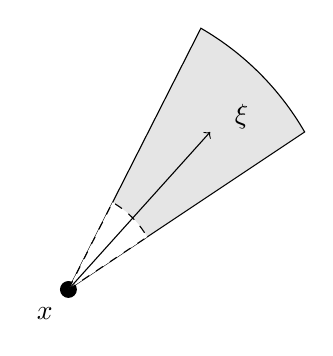
\begin{tikzpicture}
    \draw [fill=black] (0, 0) circle [radius=0.1]; \node at (-0.3, -0.3) {$x$}; 
    
    \filldraw[fill=gray!20!white]
    (0,0) -- (3, 2) arc (30:60:3.6) -- (0,0);
    
    \filldraw[fill=white!20!white, dashed]
    (0,0) -- (1, 0.66666) arc (30:60:1.2) -- (0,0);
    
    \draw [-> ] (0, 0) -- (1.8, 2); \node at (2.2, 2.2) {$\xi$};
    \end{tikzpicture}
    \captionof{figure}{Microlocalisation in phase space. }
\end{center}

\begin{fdefinition}
    The \textbf{wavefront set} of a compactly supported tempered distribution 
    \[
    u \in C^{-\infty}_c(\R^n) = \set{u \in \sch'(\R^n) \wh \supp(u) \Subset \R^n} 
    \]
    is given by 
    \begin{align*}
    \WF(u) = \bigcap \set{\Char^0(A) \wh A \in \Psi^0_\infty(\R^n), Au \in C^\infty(\R^n)}. 
    \end{align*}
    For general tempered distribution $u \in \sch'(\R^n)$, its wavefront set is given by 
    \begin{align*}
    \WF(u) = \bigcup_{\chi \in C^\infty_c(\R^n)} \WF(\chi u). 
    \end{align*}
\end{fdefinition} 



\section{Fredholm problem for the wave operator on torus} 

\begin{definition} 
    Let $\S^1 = [0,1] / (0 \sim 1)$ denote the circle and for any $k \in \N$ let
    \begin{align*}
    \T^k := \underbrace{\S^1 \times \S^1 \times \dots \times \S^1}_{k}
    \end{align*}
    denote the $k$-dimensional torus. We shall study the totally periodic wave operator, on $M :=  = \T_t^1 \times \T_x^{n}$ given by
    \begin{align}\label{eq: d'Alembertian}
    \Box := \p_t^2 - \sum_{j = 1}^{n -1} \p_{x_j}^2
    \end{align}
    where $(t, x_1, \dots, x_n)$ are the local coordinates on $M$. 
\end{definition}


%------------------------------------------------ Section : Speech 
\pagebreak
\section{Speech script} 



%------------------------------------------------ Edn


\pagebreak 
\appendix
\section{Notes:}
%From Vasy's talk (youtube: non-elliptic fredholm problem): 
"propagation of singularity" is one of the most basic phenomenon in non-elliptic setting (connected microlocal energy esitmates). If $P \in \Psi^{m}_{\infty}(\R^n)$, with real homogeneous principal symbol
\begin{itemize}
    \item $\WF^s(u)$ measures if $u$ is microlocally in $H^s$. $\alpha \not \in \WF^s(u) \iff $ there is $A \in \Psi^{0}_{\infty}(\R^n)$ elliptic at $\alpha$ and $Au \in H^s$. 
    \item Away from $\Char^m(P)$, we have microlocal elliptic regularity, i.e. $\WF^s(u) \setminus \Char(P) \subset \WF^{s - m}(Pu)$. 
    \item In $\Char^m(P) \setminus \WF^{s - m + 1}(Pu)$, however, $\WF^s(u)$ is a union of maximally extended bicharacteristics. (Closed graph theorem gives estimates, estimates about both regularity and decay) (complex absorption is an option to control the initial regularity estimate on the right hand side of the inequality.)
\end{itemize}


Generalisation to Pseudodifferential operators. Keeping concepts like symbols and principal symbols, wave front set. Theorems go through. Generalisation to manifold (problem with compactness. Need decay). 

Wave operator are typical of hyperbolic equations. 




\subsection{alternative for elliptic differential operators} 
To illustrate, we consider constant coefficient differential operator of order $m$
\begin{align*}
P = \sum_{\abs{\alpha} \leq m} c_\alpha D^\alpha_x, \quad c_\alpha \in \C
\end{align*}
It can be shown that an $m^{th}$ order differential operator defines a continuous (i.e. bounded) map 
\begin{align*}
P : H^{s}(\R^n) \to H^{s - m}(\R^n)
\end{align*}
that is, we decrease the order of regularity by $m$. The symbol of $P$ is the the polynomial 
\begin{align*}
p(\xi) = \sum_{\abs{\alpha} \leq m} c_\alpha \xi^\alpha 
\end{align*}
which is precisely the polynomial that makes the following square commutes
%\begin{center}
%    \begin{tikzcd}
%    &\sch(\R^n) \ar[r, "P"] \ar[d, "\F", "\cong"'] & \sch(\R^n) \ar[d, "\F", "\cong"'] \\
%    &\sch(\R^n) \ar[r, "p(\xi)"')] & \sch(\R^n) 
%    \end{tikzcd}
%\end{center}
i.e. 
\begin{align*}
\F Pu  = p(\xi) \F u  \quad u \in \sch(\R^n) 
\end{align*}
Question: When is the map above surjective? Answer: When it is elliptic. 

\begin{theorem}
    Let $P$ be an order $m$ differential operator. If for some $\epsilon > 0$, $p(\xi)$ above satisfies
    \begin{align*}
    \abs{p(\xi)} \geq \epsilon \brac{ 1 + \abs{\xi}^2}^{m / 2} \quad \text{ whenever } \abs{\xi} > 1/\epsilon, 
    \end{align*}
    we say $p(\xi)$ and therefore $P$ are elliptic of order $m$ and as a map
    \begin{align*}
    P: H^{s}(\R^n) \to H^{s - m}(\R^n)
    \end{align*}
    $P$ is surjective. 
\end{theorem}
\todo{show graph of $p(\xi)$ bounded below by polynomial outside of a initial compact set} \\

The statement is actually a statement of the principal part of the symbol only. 
\begin{lemma}
    A polynomial of order $m$, $p(\xi) = \sum_{\abs{\alpha} \leq m} c_\alpha \xi^\alpha$ is elliptic of of order $m$ if and only if its leading part is never zero except perhaps at $\xi = 0$, i.e. 
    \begin{align*}
    p_m(\xi) := \sum_{\abs{\alpha} = m} c_\alpha \xi^\alpha \neq 0 
    \end{align*}
    for any $\xi \neq 0$. 
\end{lemma}
\end{document}